\begin{figure*}
 \begin{tabular}{MM*5{C}@{}}
 & & noise free  & $\sigma_1=253$ & $\sigma_2=146$ & $\sigma_3=80$ & $\sigma_4=46$ \\ 
\multirow{2}{*}{\rotatebox[origin=c]{90}{beta reconstruction\hspace*{1cm} }} & \rotatebox[origin=c]{90}{ standard }  & 
\includegraphics[width=0.19\textwidth]{{fig3/beta_st_noiseFalse_ang400_shift4_maxint3}.png} & 
\includegraphics[width=0.19\textwidth]{{fig3/beta_st_noiseTrue_ang400_shift4_maxint3}.png} & 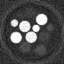
\includegraphics[width=0.19\textwidth]{{fig3/beta_st_noiseTrue_ang400_shift4_maxint1}.png} & 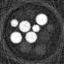
\includegraphics[width=0.19\textwidth]{{fig3/beta_st_noiseTrue_ang400_shift4_maxint0.3}.png} & 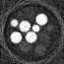
\includegraphics[width=0.19\textwidth]{{fig3/beta_st_noiseTrue_ang400_shift4_maxint0.1}.png}\\ 
& \rotatebox[origin=c]{90}{ joint $\rho=0$ }  & 
\includegraphics[width=0.19\textwidth]{{fig3/beta_joint0_noiseFalse_ang400_shift4_maxint3}.png} & 
\includegraphics[width=0.19\textwidth]{{fig3/beta_joint0_noiseTrue_ang400_shift4_maxint3}.png} & 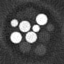
\includegraphics[width=0.19\textwidth]{{fig3/beta_joint0_noiseTrue_ang400_shift4_maxint1}.png} & 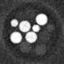
\includegraphics[width=0.19\textwidth]{{fig3/beta_joint0_noiseTrue_ang400_shift4_maxint0.3}.png} & 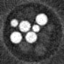
\includegraphics[width=0.19\textwidth]{{fig3/beta_joint0_noiseTrue_ang400_shift4_maxint0.1}.png}\\ 
& \rotatebox[origin=c]{90}{ joint $\rho=0.5$ }  & 
\includegraphics[width=0.19\textwidth]{{fig3/beta_joint_noiseFalse_ang400_shift4_maxint3}.png} & 
\includegraphics[width=0.19\textwidth]{{fig3/beta_joint_noiseTrue_ang400_shift4_maxint3}.png} & 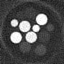
\includegraphics[width=0.19\textwidth]{{fig3/beta_joint_noiseTrue_ang400_shift4_maxint1}.png} & 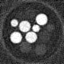
\includegraphics[width=0.19\textwidth]{{fig3/beta_joint_noiseTrue_ang400_shift4_maxint0.3}.png} & 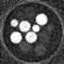
\includegraphics[width=0.19\textwidth]{{fig3/beta_joint_noiseTrue_ang400_shift4_maxint0.1}.png}\\ 
\multirow{2}{*}{\rotatebox[origin=c]{90}{delta reconstruction\hspace*{1cm} }} & \rotatebox[origin=c]{90}{ standard }  & 
\includegraphics[width=0.19\textwidth]{{fig3/delta_st_noiseFalse_ang400_shift4_maxint3}.png} & 
\includegraphics[width=0.19\textwidth]{{fig3/delta_st_noiseTrue_ang400_shift4_maxint3}.png} & 
\includegraphics[width=0.19\textwidth]{{fig3/delta_st_noiseTrue_ang400_shift4_maxint1}.png} & 
\includegraphics[width=0.19\textwidth]{{fig3/delta_st_noiseTrue_ang400_shift4_maxint0.3}.png} & 
\includegraphics[width=0.19\textwidth]{{fig3/delta_st_noiseTrue_ang400_shift4_maxint0.1}.png}\\ 
& \rotatebox[origin=c]{90}{ joint $\rho=0$ }  & 
\includegraphics[width=0.19\textwidth]{{fig3/delta_joint0_noiseFalse_ang400_shift4_maxint3}.png} & 
\includegraphics[width=0.19\textwidth]{{fig3/delta_joint0_noiseTrue_ang400_shift4_maxint3}.png} & 
\includegraphics[width=0.19\textwidth]{{fig3/delta_joint0_noiseTrue_ang400_shift4_maxint1}.png} & 
\includegraphics[width=0.19\textwidth]{{fig3/delta_joint0_noiseTrue_ang400_shift4_maxint0.3}.png} & 
\includegraphics[width=0.19\textwidth]{{fig3/delta_joint0_noiseTrue_ang400_shift4_maxint0.1}.png}\\ 
& \rotatebox[origin=c]{90}{ joint $\rho=0.5$}  & 
\includegraphics[width=0.19\textwidth]{{fig3/delta_joint_noiseFalse_ang400_shift4_maxint3}.png} & 
\includegraphics[width=0.19\textwidth]{{fig3/delta_joint_noiseTrue_ang400_shift4_maxint3}.png} & 
\includegraphics[width=0.19\textwidth]{{fig3/delta_joint_noiseTrue_ang400_shift4_maxint1}.png} & 
\includegraphics[width=0.19\textwidth]{{fig3/delta_joint_noiseTrue_ang400_shift4_maxint0.3}.png} & 
\includegraphics[width=0.19\textwidth]{{fig3/delta_joint_noiseTrue_ang400_shift4_maxint0.1}.png}\\ 
\end{tabular}
 \caption{Reconstruction. obj size=(15,64,64), voxelsize=1.0e-06, prb size = 15, ang=400, shift=4, joint (piter,titer,NITER)=(4,4,50), standard (piter,titer,NITER)=(200,200,1)} 
 \end{figure*} 